\subsection{Perlin Noise}

A técnica de Perlin Noise é um algoritmo de geração de ruído procedural, que cria padrões aleatórios, porém coerentes e orgânicos. Ao contrário de um ruído puramente aleatório (também conhecido como "ruído branco"), que gera valores sem correlação, o Perlin Noise produz transições suaves e graduais.

O algoritmo baseia-se em um grid regular de pontos no espaço, onde a cada nó do grid é atribuído um vetor gradiente pseudo-aleatório. Estes vetores são gerados por uma função hash (ou uma tabela de permutações), que garante que a mesma coordenada de nó sempre retorne o mesmo vetor.

Para calcular o valor do ruído em qualquer ponto do espaço, o algoritmo segue três passos principais:
\begin{enumerate}
    \item Calcula-se o produto interno (dot product) entre o vetor de deslocamento do ponto de interesse até cada nó do grid e o vetor gradiente pseudo-aleatório de cada nó. O produto interno mede a projeção do ponto na direção do vetor gradiente.
    \item Os valores obtidos são então suavizados usando uma função de interpolação cúbica, como $3x^2 - 2x^3$. Esta função assegura que a transição entre as células do grid seja contínua e suave, evitando arestas visíveis e criando a aparência orgânica característica do Perlin Noise.
    \item Os valores suavizados são interpolados (bilinearmente em 2D ou trilinearmente em 3D) para obter o valor final no ponto.
\end{enumerate}

O resultado é um campo de valores que varia suavemente, ideal para simular texturas naturais como nuvens, fogo e terrenos. A Figura \ref{fig:whitenoise} demonstra a diferença visual entre o \textit{Value Noise} (que usa interpolação linear) e o \textit{Perlin Noise} (que usa interpolação cúbica) \cite{fractalNoise}.

\begin{figure}[H]
    \centering
    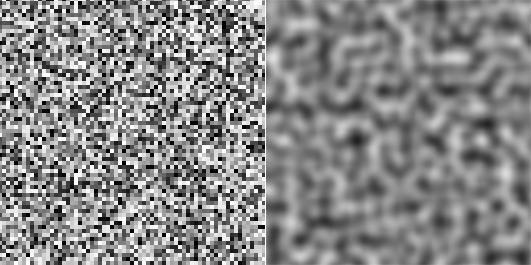
\includegraphics[width=0.8\linewidth]{img/noise-whitenoise.png}
    \caption{Diferença entre \textit{Value Noise} (à esquerda) e \textit{Perlin Noise} (à direita).}
    \label{fig:whitenoise}
\end{figure}

Em um espaço vetorial de coordenadas inteiras $[x, y, z]$, uma função hash $H()$ é utilizada para mapear cada coordenada a um valor pseudo-aleatório. Essa função é essencial para a reprodutibilidade do ruído.

Uma vez que o valor de ruído $Noise([x, y, z])$ é calculado, ele pode ser interpretado como um sinal para a modulação de cores, posições ou outras propriedades de um objeto. A aplicação do ruído pode gerar perturbações em texturas, como visto nas Figuras \ref{fig:donut_noise}, \ref{fig:sphere_noise} e \ref{fig:cube_noise}.

\begin{figure}[H]
    \centering
    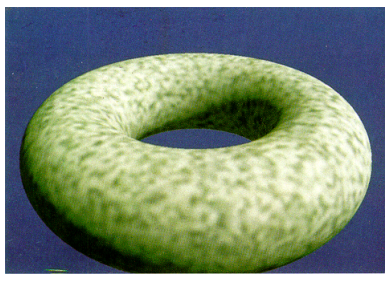
\includegraphics[width=0.4\textwidth]{img/donut.png}
    \caption{Donut com textura Noise aplicada}
    \label{fig:donut_noise}
\end{figure}

\begin{figure}[H]
    \centering
    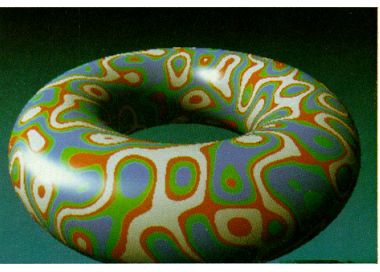
\includegraphics[width=0.4\textwidth]{img/donut2.png}
    \caption{Esfera com textura Noise aplicada}
    \label{fig:sphere_noise}
\end{figure}

\begin{figure}[H]
    \centering
    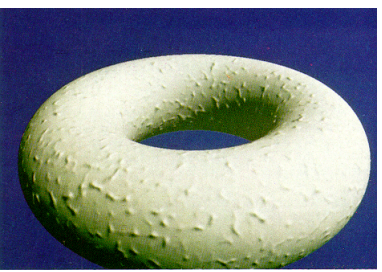
\includegraphics[width=0.4\textwidth]{img/donut3.png}
    \caption{Cubo com textura Noise aplicada}
    \label{fig:cube_noise}
\end{figure}

A derivada do Perlin Noise, chamada de Dnoise(), é o vetor diferencial do ruído e representa a taxa de variação instantânea do ruído em cada uma das três direções do espaço. A aplicação do Dnoise() permite a criação de perturbações de superfície, influenciando, por exemplo, a normal de um objeto para simular relevo e detalhes finos.

$$
\text{normal} += \text{Dnoise}(\text{array})
$$

\begin{figure}[H]
    \centering
    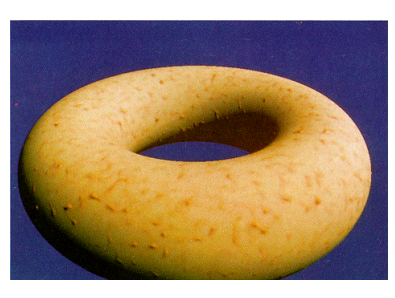
\includegraphics[width=0.4\textwidth]{img/donut4.png}
    \caption{Donut com textura Dnoise aplicada}
    \label{fig:donut_dnoise}
\end{figure}

Como estes cálculos são aplicados a nível de pixel em \textit{shaders}, a taxa de amostragem é fundamental. Frequências mais altas que a frequência de amostragem podem causar aliasing, um efeito indesejado. Para mitigar isso, as amostras são feitas de modo que a frequência do ruído se mantenha apropriada para a resolução do pixel.

O autor descreve uma técnica para simular a aparência de mármore usando a função \texttt{Noise()}. O método parte do princípio de que a aparência do mármore resulta de camadas heterogêneas que foram deformadas por forças turbulentas antes de se solidificarem. A abordagem é, portanto, uma combinação de uma estrutura regular e simples (as camadas) com uma complexa estrutura estocástica (o ruído da turbulência). A base do modelo são as camadas, representadas por uma simples onda senoidal, \texttt{sin(x)}. O autor usa a coordenada \texttt{point[1]} como o input para essa função, e o valor resultante é então mapeado para cores através de uma função auxiliar \texttt{marble\_color()}. Para adicionar o realismo das forças turbulentas, o autor introduz uma função \texttt{turbulence()}. Esta função é usada para perturbar a coordenada de entrada \texttt{x} antes que ela seja passada para a onda senoidal. O pseudocódigo que combina esses elementos é o seguinte:

\begin{lstlisting}[language=Python, caption={Pseudocódigo da função marble()}]
def marble(point):
  x = point[1] + turbulence(point)
  return marble_color(sin(x))
\end{lstlisting}

A função \texttt{turbulence()} é, por sua vez, uma soma de ruído em diferentes escalas, um processo que cria um padrão auto-semelhante ou \textit{1/f}. O algoritmo para a \texttt{turbulence()} é detalhado como:

\begin{lstlisting}[language=Python, caption={Pseudocódigo da função turbulence()}]
def turbulence(p):
  t = 0
  scale = 1
  while (scale > pixelsize):
    t += abs(Noise(p / scale) * scale)
    scale *= 2
  return t
\end{lstlisting}

Este procedimento garante que a quantidade de ruído adicionada em cada escala seja proporcional ao seu tamanho, resultando na impressão visual de movimento browniano. Além disso, o uso da função \texttt{abs()} em cada iteração assegura que o gradiente da textura tenha limites descontínuos em todas as escalas, o que é interpretado visualmente como fluxo turbulento.

\begin{figure}[H]
    \centering
    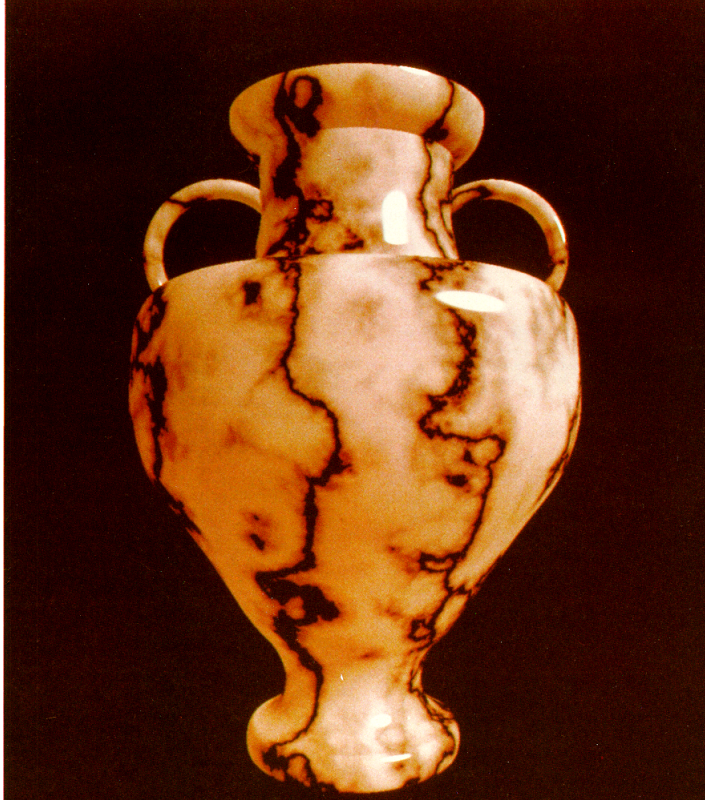
\includegraphics[width=0.4\textwidth]{img/marble.png}
    \caption{Textura de mármore gerada com a função marble()}
    \label{fig:marble_texture}
\end{figure}


\subsubsection{Mapeamento de Texturas Sólidas}
Qualquer função que mapeie um domínio de dimensões espaciais (como $\mathbb{R}^3$) para um valor (cor, por exemplo) pode ser considerada uma "função espacial". A partir disso, cada função espacial pode ser interpretada como a representação de um material sólido.

Desta forma, ao avaliar estas funções nos pontos visíveis da superfície de um objeto, é possível obter a textura da superfície, de modo parecido a ter "contornado" o objeto com o material. A textura obtida a partir deste tipo de extração é frequentemente tratada como uma textura sólida. Este termo é usado para descrever a representação de materiais que preenchem um volume, em vez de estarem apenas na superfície \cite{fractalNoise}.

\subsection{Ruído Fractal ou \textit{Fractional Browmian Motion} (fBm)}

A base para a geração procedural de terrenos é a criação de um mapa de alturas (\textit{heightmap}), onde o valor de brilho de um pixel corresponde à altitude de um ponto em um terreno. Um único ruído coerente, como o Perlin, gera um relevo excessivamente suave, como colinas perfeitamente arredondadas. Para criar a complexidade e os detalhes em múltiplas escalas de uma paisagem natural, o Ruído Fractal é aplicado.

A técnica consiste em somar várias camadas de ruído (chamadas de \textbf{oitavas}), cada uma contribuindo com um nível diferente de detalhe para a altitude final do terreno.

\begin{equation*}
\text{Altitude}(x, z) = \sum_{i=0}^{n-1} \text{amplitude}_i \cdot \text{Ruído}(\text{frequência}_i \cdot (x, z))
\end{equation*}

Os parâmetros que controlam a aparência do terreno são:
\begin{itemize}
\item \textbf{Oitavas (n):} O número de camadas de detalhe. As primeiras oitavas definem as cordilheiras principais e os vales. As últimas oitavas adicionam a rugosidade da superfície, como rochas e solo irregular.
\item \textbf{Lacunaridade (L):} Controla o aumento da frequência a cada oitava (tipicamente 2.0). Em termos práticos, define quão rapidamente os detalhes ficam menores. Uma lacunaridade alta cria terrenos com uma transição brusca entre as feições grandes e a rugosidade fina.

\item \textbf{Persistência (P):} Controla a diminuição da amplitude a cada oitava (tipicamente 0.5). Este é o parâmetro mais importante para o "sentimento" do terreno. Uma persistência baixa ($<0.5$) cria terrenos mais suaves e erodidos, onde as formas principais dominam. Uma persistência alta ($>0.5$) resulta em terrenos mais caóticos e rochosos, com grande influência dos detalhes finos.

\end{itemize}

\subsubsection{Criando Terrenos Rochosos com Ruído Turbulento}
Para modelar terrenos com características mais abruptas, como montanhas escarpadas ou cânions, uma variação chamada \textbf{Turbulência} é utilizada. Em vez de somar o ruído diretamente, somamos seu valor absoluto.
\begin{equation*}
\text{Altitude}{\text{turbulenta}}(x, z) = \sum{i=0}^{n-1} \text{amplitude}_i \cdot |\text{Ruído}(\text{frequência}_i \cdot (x, z))|
\end{equation*}
Esta simples modificação transforma os vales suaves em cumes afiados e ravinas, conferindo um aspecto mais "quebrado" e agressivo à paisagem, ideal para terrenos rochosos e vulcânicos.

\subsubsection{Simulando Erosão e Feições Orgânicas com Distorção de Domínio}
Para criar paisagens mais realistas e orgânicas, como vales de rios sinuosos ou padrões de erosão, a técnica de \textbf{Distorção de Domínio} (\textit{Domain Warping}) é aplicada. A ideia é usar uma função de ruído para "deformar" as coordenadas de entrada de outra.

Por exemplo, a altitude de um ponto (x,z) não é calculada diretamente. Primeiro, calculamos um deslocamento usando outro ruído:
\begin{align*}
    \text{deslocamento}_x &= C \cdot \text{fBm}_1(x, z) \\
    \text{deslocamento}_z &= C \cdot \text{fBm}_2(x, z)
\end{align*}
E então usamos as coordenadas distorcidas para calcular a altitude final:
\begin{equation*}
\text{Altitude}(x, z) = \text{fBm}{\text{base}}(x + \text{deslocamento}_x, z + \text{deslocamento}_z)
\end{equation*}
O resultado são terrenos com feições que parecem fluir e se conectar de maneira natural, simulando o efeito de forças como água e vento esculpindo a paisagem ao longo do tempo.

\subsection{O Algoritmo Diamond-Square}

Enquanto o Ruído Fractal (fBm) constrói um terreno somando ruídos em diferentes escalas (uma abordagem \textit{bottom-up}), o algoritmo \textbf{Diamond-Square} gera terrenos fractais através de um processo de subdivisão recursiva (uma abordagem \textit{top-down}). Ele opera sobre um grid quadrado cujas dimensões devem ser uma potência de dois mais um (ex: $2^n + 1$).

O algoritmo é inicializado com valores de altitude nos quatro cantos do grid e, em seguida, itera através de dois passos principais até que todo o grid seja preenchido:

\begin{enumerate}
    \item \textbf{Passo Diamante (Diamond Step):} Para cada quadrado no grid, o ponto central (o "diamante") recebe um valor de altitude que é a média dos quatro cantos do quadrado, acrescido de um pequeno deslocamento aleatório.

    \item \textbf{Passo Quadrado (Square Step):} Para cada diamante recém-criado, o ponto central de cada uma das suas quatro arestas (formando um "quadrado" rotacionado) recebe um valor de altitude. Esse valor é a média dos pontos vizinhos do diamante, acrescido de um deslocamento aleatório. Para os pontos nas bordas do grid, a média é calculada com apenas três pontos vizinhos.

    \item \textbf{Recorrência:} A cada iteração, a magnitude do deslocamento aleatório é reduzida. O processo é repetido para os novos quadrados menores que foram formados, até que todos os pontos do grid tenham um valor de altitude.
\end{enumerate}

O Diamond-Square é um método clássico, rápido e relativamente simples de implementar. No entanto, sua principal desvantagem é a tendência a gerar artefatos visuais, como cumes e vales alinhados com os eixos X e Y do grid, algo que o Perlin Noise evita naturalmente.

\subsection{Pós-Processamento e Realismo através da Simulação de Erosão Hidráulica}

Os terrenos gerados por algoritmos puramente matemáticos, como o fBm ou o Diamond-Square, muitas vezes carecem do realismo forjado por milênios de forças naturais. Para preencher essa lacuna, aplicamos algoritmos de simulação física como um passo de pós-processamento, sendo a erosão hidráulica um dos mais impactantes.

Essa técnica simula o efeito da água escoando sobre a superfície do terreno, esculpindo-o de forma natural. Um modelo comum é baseado na simulação de partículas (gotículas de chuva):

\begin{itemize}
    \item \textbf{Criação:} Milhares de "gotas d'água" são simuladas, cada uma sendo posicionada em um ponto aleatório do terreno.

    \item \textbf{Escoamento:} A gota calcula o gradiente de altitude ao seu redor e move-se para o vizinho mais baixo, simulando o fluxo da água morro abaixo.

    \item \textbf{Erosão:} À medida que a gota se move e ganha velocidade, ela "erode" uma pequena quantidade de sedimento do terreno, diminuindo a altitude dos pontos por onde passa.

    \item \textbf{Transporte e Deposição:} A gota carrega o sedimento consigo. Quando sua velocidade diminui (por exemplo, ao atingir uma área mais plana), ela perde a capacidade de carregar o material e o "deposita", aumentando a altitude do terreno naquele local.

    \item \textbf{Evaporação:} Após um certo tempo ou distância percorrida, a gota "evapora", e o ciclo recomeça com uma nova gota.
\end{itemize}

O resultado final é um terreno muito mais convincente, com a formação de redes de rios, vales suavizados, ravinas íngremes e planícies de aluvião, características que são extremamente difíceis de gerar apenas com funções de ruído \cite{erosion}.
